\newcommand{\novp}{\textit{\textbf{SFNoVP}}}
\newcommand{\vp}{\textit{\textbf{SFVP}}}
\newcommand{\nfnovp}{\textit{\textbf{RRFNoVP}}}
\newcommand{\nfvp}{\textit{\textbf{RRFVP}}}

\newcommand{\optvp}{\textit{\textbf{OptVP}}}
\newcommand{\vt}{\textit{\textbf{VT}}}
\newcommand{\nfvt}{\textit{\textbf{RFVT}}}
\vspace{-1em}

%This chapter demonstrates that modifying the hardware to improve the performance of core composition requires modifying the systems.
%The modifications discussed in the chapter are better branch prediction, adding a value predictor, and modifying the block fetching scheme.
%Whilst a value predictor improves performance by allowing blocks to execute in parallel via speculating register values, value predictors are still considered a work in progress~\cite{peraisBeBop2015}.
%It is important to consider how a perfect system with the new hardware additions can improve the performance of core composition, as it gives an upper bound to the potential performance increases.

This section explores how a perfect branch and value predictor, paired with the new fetching scheme, improves the performance of core composition on the SD-VBS benchmarks.
To understand how each component contributes to the performance improvements, different configurations were used, they are as follows:
\begin{itemize}
\item Serial fetching scheme with no value prediction (\novp).
\vspace{-1em}
\item Serial fetching scheme with perfect value prediction (\vp).
\vspace{-1em}
\item Round robin fetching scheme with no value prediction (\nfnovp).
\vspace{-1em}
\item Round robin fetching scheme with value prediction (\nfvp).
\end{itemize}

All configurations use perfect branch prediction as to ensure that core composition is always on the correct execution path.
All benchmarks are executed with 16 cores composed as this is the maximum number of cores that can be fused.
No dynamic adaptation is done as Chapter~\ref{chp:cases} showed that the primary advantage of dynamic core composition is energy savings, whereas this chapter focuses on speedup.


\subsection{Analysing the performance of the different configurations}
Figure~\ref{fig:perf_pred} shows the speedup obtained on the SD-VBS benchmarks using the different configurations.
The baseline for this section is normal fetching scheme with no value prediction (\novp) with perfect branch prediction.
This baseline is chosen as this chapter is focused on improving the performance of core composition.


First, it is clear that using the round robin fetching scheme (RRF) with value prediction (\nfvp) always results in the best speedup compared to the baseline.
For \bm{Multi\_NCut}, performance is improved by 3x when using \nfvp.
This is a significant speedup, as Chapter~\ref{chp:cases} showed that \bm{Multi\_Ncut} is a difficult benchmark for core composition (1.3x speedup in Chapter~\ref{chp:cases}).
On average, \nfvp{} outperforms the baseline by a factor of 1.88x.

\begin{figure}[t]
    \centering
    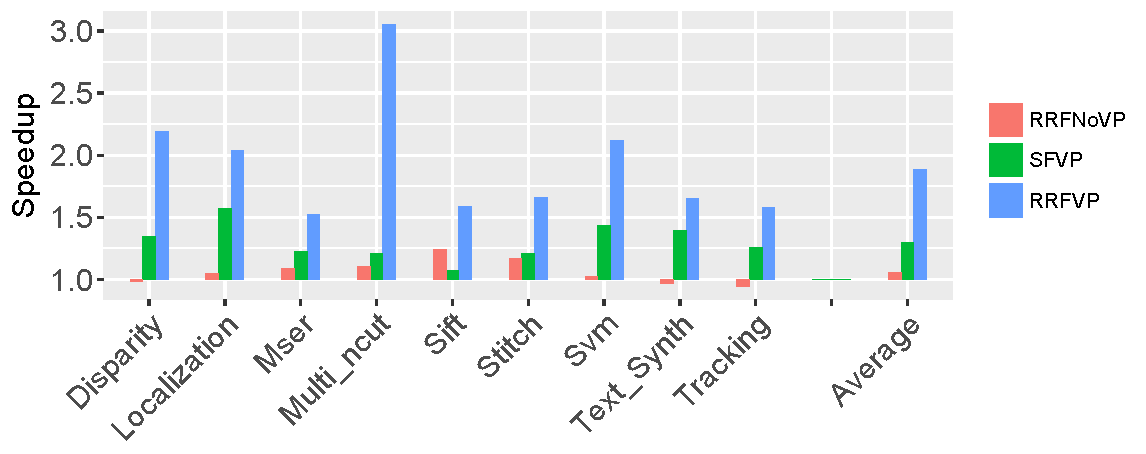
\includegraphics[width=1\textwidth]{chapter3/graphics/tempres4.pdf}
    \caption{Comparing the performance of serial fetch to round robin fetch, with and without perfect value prediction. Higher is better}
    \label{fig:perf_pred}
\end{figure}

\subsubsection{Performance without value prediction}
The results in Figure~\ref{fig:perf_pred} show that without value prediction the performance improvements brought by RRF on its own are almost non-existant, or in fact detrimental to performance.
For example, \bm{Multi\_NCut} only has a 1.10x speedup when using the \nfnovp{} configuration, compared to the 3x of \nfvp{}.
This is due to the fact that whilst more blocks are now spread across cores, the register dependencies between blocks limit the performance of the composition. 
The performance limitations are caused by blocks that are further down the speculative path that must wait for older blocks to write to the register file.
In fact, the more even distribution is the reason why some benchmarks perform worse: \bm{Disparity}, \bm{Texture\_Synthesis} and \bm{Tracking} see a slight performance decrease.
As blocks are now more evenly distributed amongst cores, this increases the stress on the network on chip (NoC) as more cores will make accesses in parallel.
This means that not only are data dependencies not resolved, but register read responses may take slightly longer to arrive as the network is saturated.
Without value prediction, RRF suffers due to NoC stress and data dependencies.
%In fact, \vp{} outperforms \nfnovp{} on \bm{Localization}, which shows that register dependencies between blocks can make the new fetching scheme less performant than the currently implemented.


\subsubsection{Performance with value prediction}
The performance improvements brought by RRF are more apparent when taking value prediction into account.
\nfvp{} has a 54\% performance increase compared to \vp{} (1.88x vs 1.22x).
The difference in performance comes from the fact that with value prediction, blocks can potentially execute faster, and thus a faster fetching scheme is required to keep up.
Since the SF scheme focuses on filling a single core, it is less likely going to benefit from parallel execution.
Even so, \vp{} results in a 1.5x speedup for \bm{Localization} which shows that value prediction is valuable for composition regardless of the scheme.

\begin{figure}[t]
    \centering
    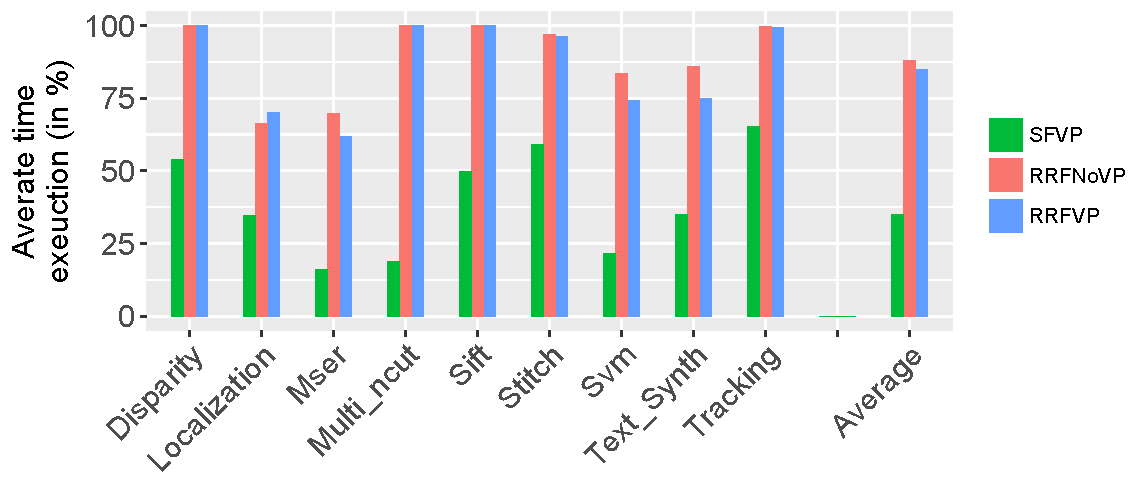
\includegraphics[width=1\textwidth]{chapter3/graphics/perf_av_cycle_exec4.pdf}
    \caption{Average time each core is executing blocks (in \%) for each benchmark, using the different configurations. Higher is better.}
    \label{fig:perf_av_cycle}
	\vspace{1em}
\end{figure}

To better highlight how the SF scheme hinders performance even with value prediction, the percentage of time a core in a composition is actively executing code, for each benchmark, is shown in Figure~\ref{fig:perf_av_cycle}.
For each configuration, the number of cycles each core in a composition has instructions to execute is averaged out and then compared to the total execution time of the application.
When the average active time of a core is close to the total execution time, this means that the composition was efficiently used, as each core had a block to run throughout the program execution.

\paragraph*{Active Cycles}
Figure~\ref{fig:perf_av_cycle} shows that \vp{} often has low active times when using a composition of 16 cores.
This is due to the fact that the SF scheme is slow, and thus, some cores are inactive, waiting to receive a fetch request from another core.
Of course, it is important to note that their LSQs and L1 caches may still be used by other active cores, simply that their execution units are not being used.
The lower the percentage is, the less likely there are going to be multiple blocks on different cores in flight which in turn means the composition is less efficient and value prediction is less useful.
Since value prediction is aimed at increasing instruction level parallelism (ILP)~\cite{peraisBeBop2015} it is important that cores may fetch blocks quickly in a composition.

With the RRF scheme, the percentage of active time is increased on average by a factor of 2.28x, and is on average 85\%.
This means that during most of the execution of an application, all cores are executing code, and thus greatly increases the chance of improving performance via core composition.
Yet, whilst cores may always have blocks to execute with RRF, it is important to remember that data dependencies and the NoC will impact performance.
It is interesting to see that \nfvp{} has a lower average time than \nfnovp{} for some benchmarks such as \bm{MSER} and \bm{Texture\_Synthesis}.
Also, whilst RRF aims to evenly distribute blocks amongst the cores, the average core utilisation for \bm{Localization} with the configurations \nfnovp{} and \nfvp{} is of 62\%.
This reduced average time is due to flushes caused by Load-Store-Queue (LSQ) violations, which causes cores to flush their instruction windows, and thus increases the number of times that cores will not be executing code.

\begin{figure}[t]
    \centering
    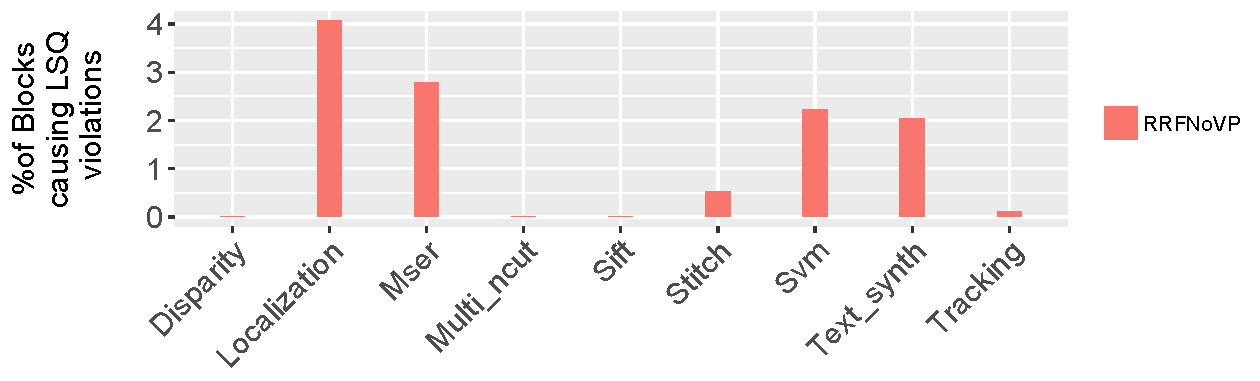
\includegraphics[width=1\textwidth]{chapter3/graphics/lsqViol4.pdf}
    \caption{Number of blocks that cause LSQ violations, normalised by the number of fetched blocks for each of the benchmarks.}
    \label{fig:lsqvio}
	\vspace{1em}
\end{figure}

Figure~\ref{fig:lsqvio} shows the number of blocks that cause an LSQ violation, normalised by the number of fetched blocks for each of the benchmarks.
For example 3\% of fetched blocks caused an LSQ violation in the benchmark \bm{MSER}.
For every LSQ violation, the entire composition may need to be flushed, and given the fact that \bm{MSER} features small blocks, refilling the entire composition may take some time, even with RRF.
Even though the percentage is quite small, it still has an impact on how efficient the composition may be, due to the fact that compositions rely on heavy speculation to obtain any performance improvements.
%A store-set dependency predictor is implemented in the processor~\cite{chrysos1998storesets}, however it is sometimes hard to predict load-store dependencies across multiple blocks, which is why LSQ violations occur.
%Store-set dependency predictors are not discussed in more detail in this chapter, however researching how store-set dependencies could be applied to core-composition is an interesting subject for future work.

\subsection{Round robin fetching scheme bottleneck Analysis}

As seen in the previous section RRF enables better use of the perfect value predictor. 
However, on its own it often does not outperform \novp{}, averaging only a speedup of 1.05x.
This section covers where the bottlenecks of RRF are, what potential solutions can be employed, and how that can improve performance overall.

\paragraph*{Block dispatching latency}

RRF improves performance of a core composition by reducing the amount of communication between cores.
This is achieved through a round robin fetching scheme, where cores do not fetch blocks sequentially, but rather in strides.
This does introduce one extra complexity: blocks that are further down the speculative path may be fetched before blocks closer to the non-speculative block.
Essentially, blocks can be fetched out of order, yet still require to be dispatched in order (recall Section~\ref{chp3:sec:fetch}).

\begin{figure}[t]
    \centering
    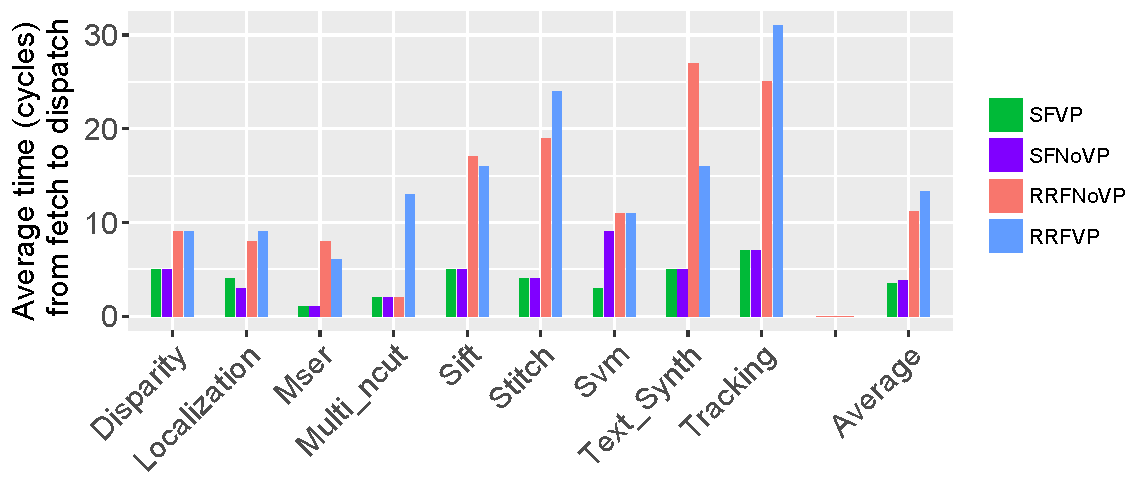
\includegraphics[width=1\textwidth]{chapter3/graphics/avTimeToFetch3.pdf}
    \caption{Average time (in cycles) for block to go from fetched to dispatched using the serial fetching scheme and round robin fetching scheme. Lower is better.}
    \label{fig:av_time}
	\vspace{1em}
\end{figure}

This means that cores may fetch blocks in their window that must wait a certain number of cycles before executing.
To understand how this affects the performance of the new fetching scheme, the average time from a block being fetched, to a block being dispatched is recorded in the simulator.
Comparing the average time between the current and new fetching scheme can provide an estimate as to how much performance is potentially lost when using RRF.

Figure~\ref{fig:av_time} shows the average time for all the SD-VBS benchmarks using the different configurations.
As can be seen, for most benchmarks, RRF's average time is 2x slower than the current.
This is due to the fact that whenever the SF scheme fetches a block, it can immediately dispatched as fetches are serialised.
Surprisingly, \bm{Multi\_NCut} for \nfvp{} has a much longer time between fetching and dispatching a block.
This is due to the fact that \bm{Multi\_NCut} features blocks of only 11 instructions on average and with value prediction blocks are committing faster than on the other configurations.
%Given that a block must access a shared counter to check if it can dispatch, and the counter can only be incremented once per cycle (atomic increment), this shared resource is causing the long fetch to dispatch latency.
Given that only one block can be dispatched per cycle, this is causing the long fetch to dispatch latency.
Even with the extra latency, RRF still ensures that every core is full, cores must now only wait for their blocks to be dispatched, rather than having for a fetch request.

\begin{figure}[t]
    \centering
    
\includegraphics[width=1\textwidth]{chapter3/graphics/fetch_ex.pdf}
    \caption{Two core composition where cores fetch blocks of varying size. Green blocks represent blocks that can be dispatched, whilst the red blocks cannot.}
    \label{fig:var_ex}
	\vspace{1em}
\end{figure}

\paragraph*{Block size variance}
Another issue that can arise when fetching with a fixed stride is that if cores are fetching blocks of different sizes this may increase the fetch to dispatch latency.
For example, in the two core composition seen in Figure~\ref{fig:var_ex} the second core fetches Block 2 that is 128 instructions.
If Block 2 were smaller, Core 2 could fetch and dispatch blocks 4 and 6.
However, since Block 2 occupies the whole instruction window, Core 2 will have to wait for block 2 to commit before doing so.
Thus blocks 5 and 7 cannot be dispatched on Core 1 before block 2 has finished executing.

Figure~\ref{fig:variance} shows the variance of block sizes in the SD-VBS benchmarks.
This was obtained by counting the different block sizes each benchmark fetched, and grouping them into 4 distinct buckets: blocks that occupy 1, 2, 3 or 4 lanes in the window.
The Figure shows that the benchmark \bm{Multi\_NCut} features a very low variance; which is why RRF has a similar fetch to dispatch latency as SF without value prediction.

%The issue of variance is not only specific to RRF, as SF will also suffer from this issue as well.
%The difference is that with SF, Core 1 would not fetch blocks 3, 5 and 7, instead it would wait for Core 2 to commit its block and submit a fetch request.
%Of course, variance only partially provides an insight as to why core composition may be less efficient; as it does not take into account data dependencies between blocks.
%Also, the variance does not take into account that blocks of different sizes may belong to different phases.
%Nevertheless, it is an important factor to take into consideration.

\begin{figure}[t]
    \centering
    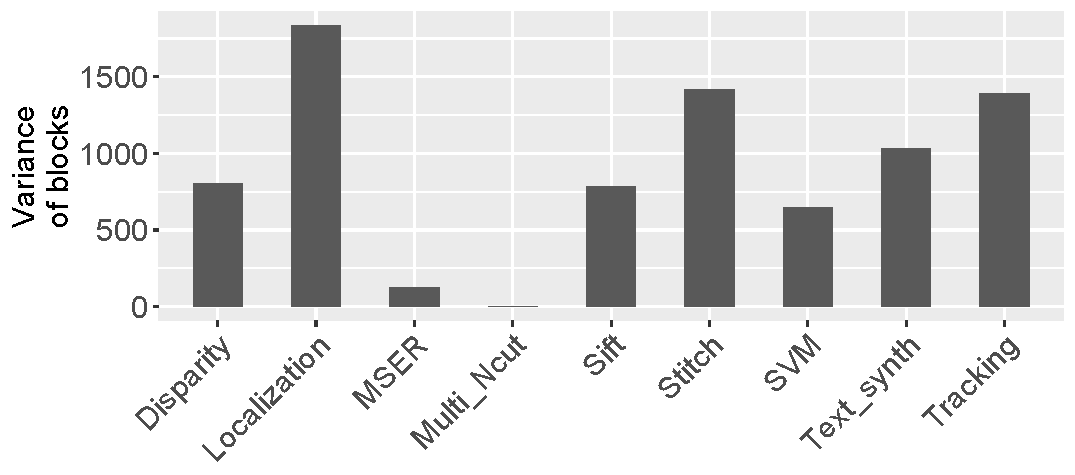
\includegraphics[width=1\textwidth]{chapter3/graphics/variance.pdf}
    \caption{Variance of block sizes per benchmark. Blocks are grouped up in buckets (occupy 1, 2, 3 or 4 segments).}
    \label{fig:variance}
	\vspace{1em}
\end{figure}

%Explain how different blcok sizes may mess up the new fetching scheme

\subsubsection{Summary}

This section shows that a perfect branch predictor, paired with perfect value prediction and the round robin fetching scheme can outperform the current configuration by a factor of up to 3x and on average a speedup of 1.87x.%, and can potentially be improved to 2.35x with further modifications to the fetching scheme.
This section also showed that without value prediction RRF only obtains a 1.09x speedup compared to the serial fetching scheme.
This is due to the fact that the benchmarks all display a certain amount of data-dependencies between blocks and that spreading blocks across cores more evenly can put pressure on the NoC; thus reduce the performance improvements of fetching blocks quicker.

